\documentclass[letterpaper, 10pt]{article}

\usepackage[english]{custompack}
\usepackage{fullpage}
%\usepackage{hyperref}
\usepackage{abcproblem}
%\renewcommand{\thesubsection}{\alph{subsection}}

%\allowdisplaybreaks
\numberwithin{theorem}{section}

\title{\textbf{untitled}}
\author{Håkon Mork \\ fagkode}
\date{\today}

\begin{document}
\section*{B \quad Overlay of Gaussian on image}
\setcounter{page}{6}
\setcounter{figure}{15}
\begin{figure}[h!]
	\centering
	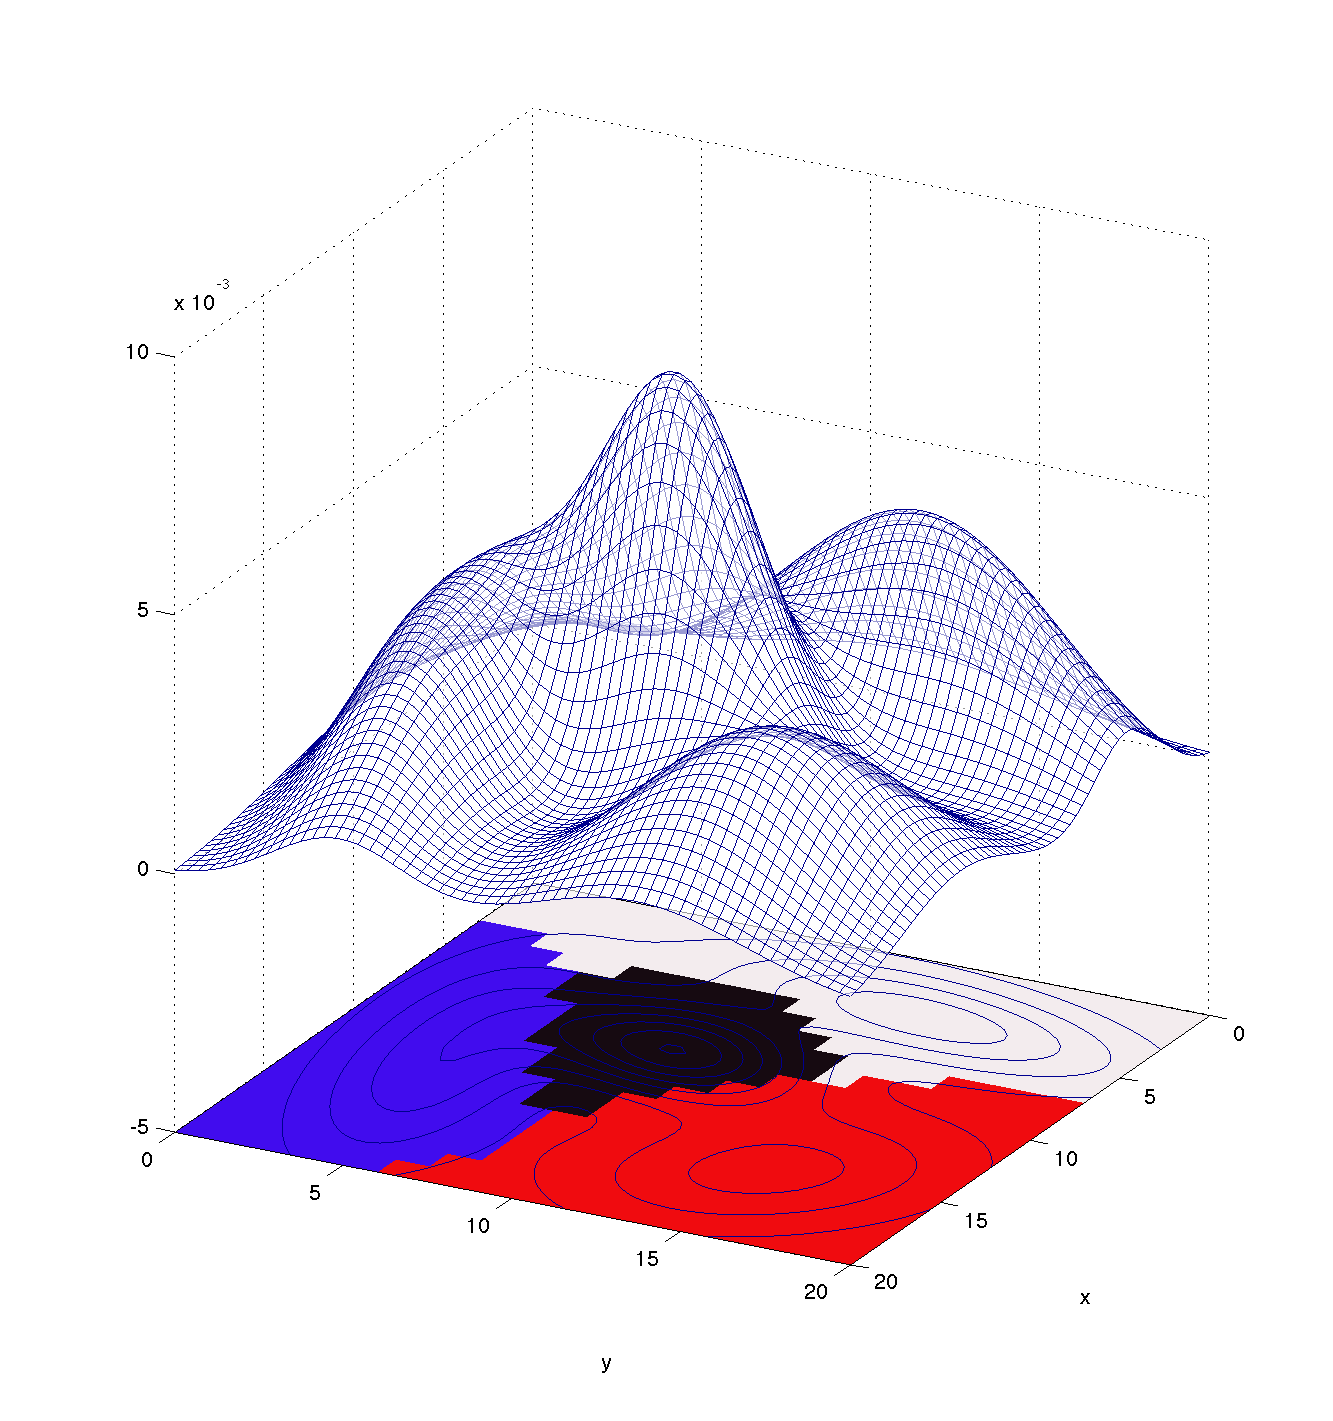
\includegraphics[width=\textwidth]{1a-gaussian}
	%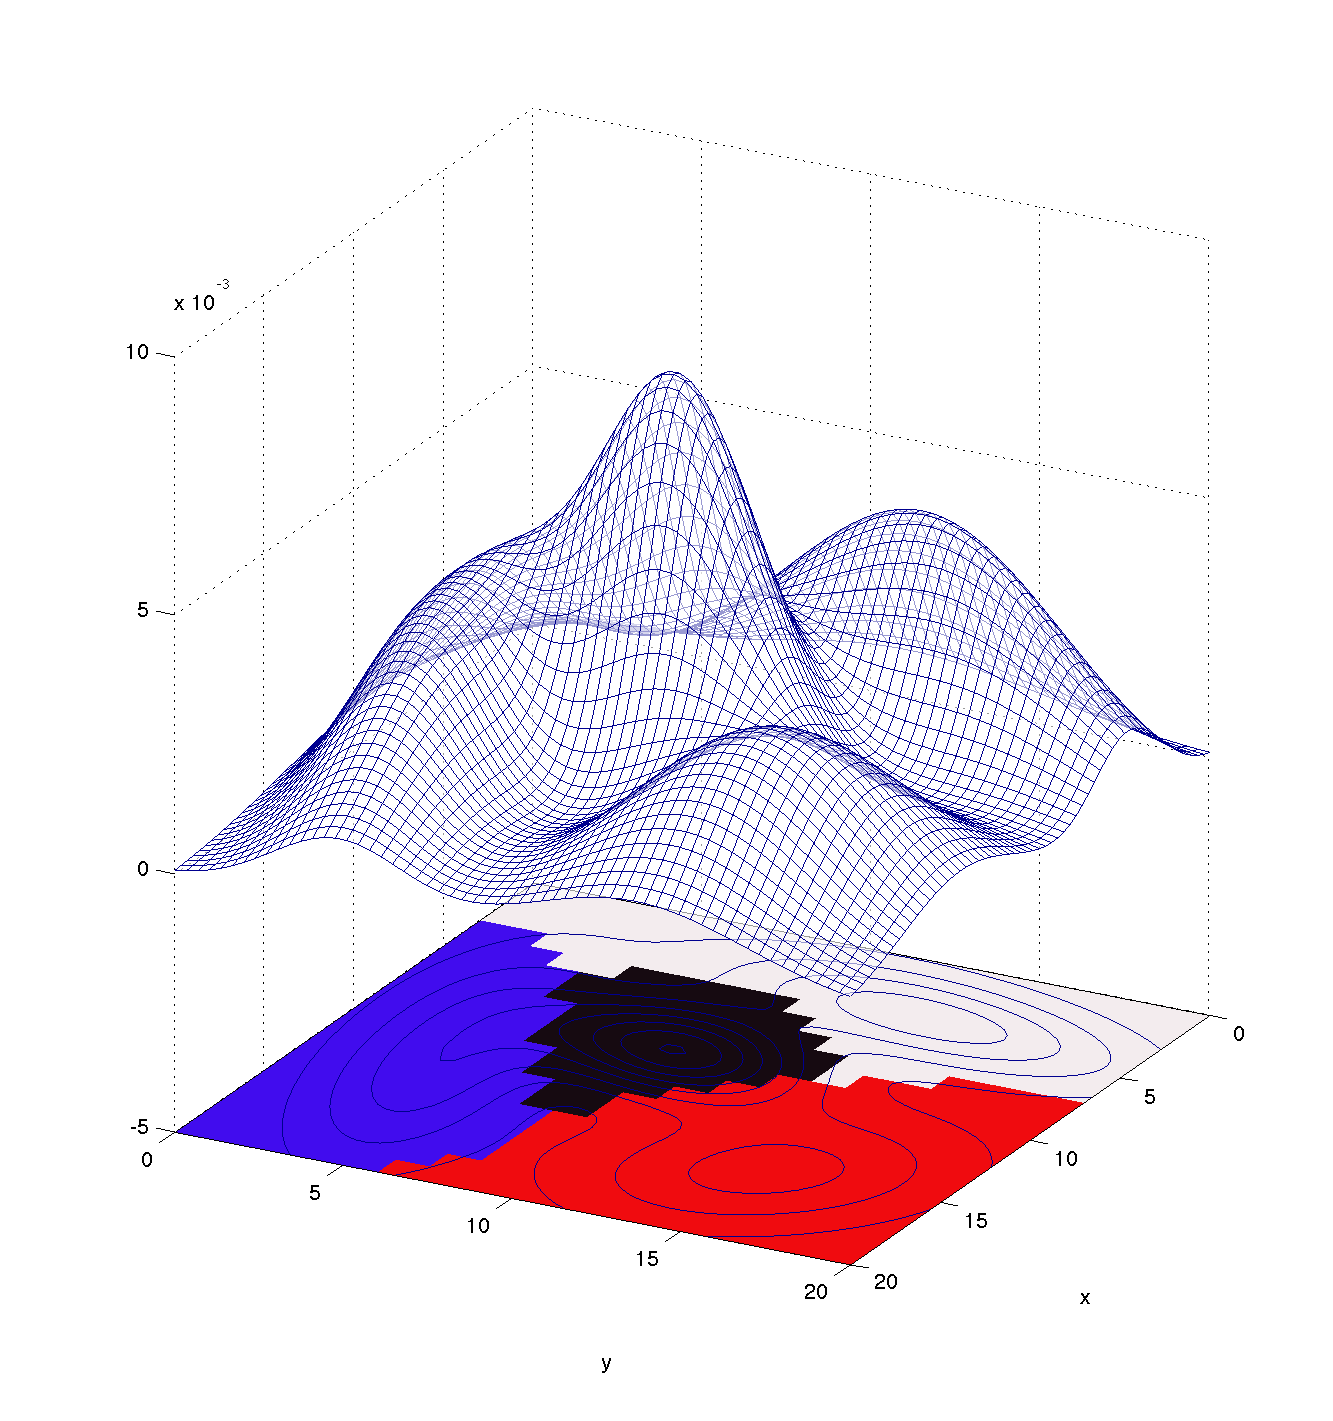
\includegraphics[height=\textheight]{1a-gaussian}
	\caption{Example of how the final Gaussian computed by the EM algorithm might look like, superimposed on image 1a. Notice how the contour lines of the Gaussian correspond nicely to the color blocks on the image. The central peak is very steep, which I guess is to ``counteract'' the influence of other nearby peaks on the small black area.}
	\label{fig:1a-gaussian}
\end{figure}

\end{document}
